\section{Functional MRI}

Many different techniques exist to accentuate different tissues, physiological phenomena etc. using MRI, of which a few will be described further in the following section. 

\subsection{Introduction to BOLD fMRI}
Functional magnetic resonance imaging measure the metabolic changes associated with different neurological tasks in different brain areas. fMRI offers advantages predominantly, high temporal and spatial resolution, low cost, and most importantly being non-invasive, which has made it a exceedingly popular method for imaging brain activity. The versatility of fMRI has made it very important tool in being a biomarker for diseases and to study the efficacy of pharmaceuticals. The method offers high resolution of anatomical structures and localization and visualization of vessels. \cite{Glover2011} 

Multiple steps in forming and transmitting a neurological signal requires energy Adenosine tripolyphosphate (ATP) consumption e.g. reception and reformation of an action potential. When activating a brain area as done in the most often used example, finger tapping, the ATP starts to be processed, leading to a decrease in oxygen concentration and increase in waste. Thereby the metabolic need for oxygen increases. As the movement is planned and executed, factors, which are present in the local tissue of the corresponding brain area, activate a vasodilation, increasing the blood flow to that area and reestablishing the local homeostasis. Though one special and not fully understood phenomenon occurs during this process. More oxygenated blood than needed to compensate for the offset is delivered. Thereby an overshoot occurs. The increase in neural activity in that specific area thereby permits two conditions which can be assessed through fMRI, being the cerebral blood flow and blood oxygen level dependent contrast. An example illustrating the measurable hemodynamic response can se found in \figref{fig:back:stim}\cite{Glover2011,Poldrack2011}

\begin{figure}[H]                 
	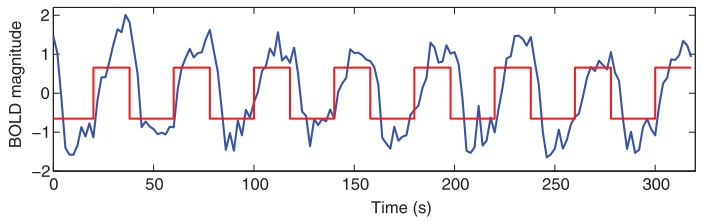
\includegraphics[width=.69\textwidth]{figures/aBackground/stimuli_vs_response}  
	\caption{Figure showing an induced series of stimuli (red) and the hemodynamic response to the neural activity measured using BOLD (blue). It is shown that the measurable hemodynamic response is delayed compared to the stimuli. \cite{Poldrack2011}}
	\label{fig:back:stim} 
\end{figure}


As established in the above section the BOLD signal is effected by the neural activity producing changes in the local blood flow, blood volume and blood oxygenation. The crucial part to why MRI can detect this natural contrast, is that fully oxygenated blood, is diamagnetic and fully deoxygenated blood has four unpaired electrons thereby making it highly paramagnetic. Thereby more oxygenated blood in the area the larger the contrast, compared to other brain regions, is seen as illustrated in \figref{fig:back:bold}. \cite{Glover2011,Khanna2015,Poldrack2011}

\begin{figure}[H]                 
	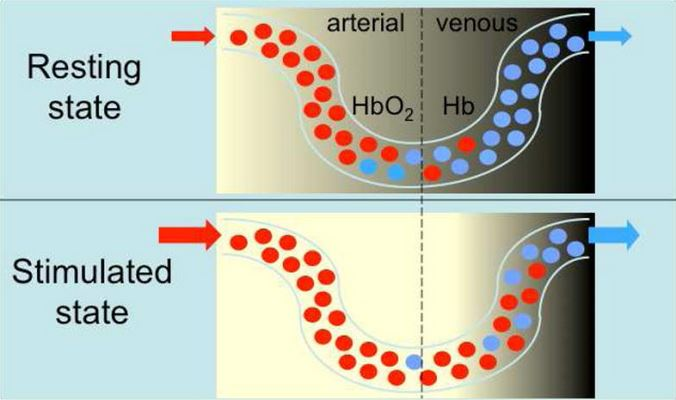
\includegraphics[width=.52\textwidth]{figures/aBackground/bold_response}  
	\caption{Illustration of how the difference in oxygen concentration in the hemoglobin change the magnetic properties, resulting in a higher measurable contrast \cite{Glover2011}.}
	\label{fig:back:bold} 
\end{figure}

This change in local magnetic properties increases the magnetic susceptibility leading to a greater MRI signal when acquiring an $T_2^*$- weighted sequence.  
